% !TEX TS-program = pdflatex
% !TEX encoding = UTF-8 Unicode

\documentclass[11pt]{article}
\usepackage[utf8]{inputenc} 
\usepackage[parfill]{parskip}
\usepackage[T1]{fontenc} 

\usepackage{polski}
\usepackage{float}
\usepackage{fixltx2e}
\usepackage{calc}
\usepackage[export]{adjustbox} % also loads graphicx
\usepackage{makeidx}
\usepackage{multicol}
\usepackage{multirow}
\PassOptionsToPackage{warn}{textcomp}
\usepackage{textcomp}
\usepackage[nointegrals]{wasysym}
\usepackage[table]{xcolor}

\usepackage{csvsimple}

% Font selection
\usepackage[T1]{fontenc}
\usepackage[scaled=.90]{helvet}
\usepackage{courier}
\usepackage{amssymb}
\usepackage{sectsty}

%%% PAGE DIMENSIONS
\usepackage{geometry} % to change the page dimensions
\geometry{a4paper} % or letterpaper (US) or a5paper or....
\geometry{margin=1in} % for example, change the margins to 2 inches all round

\usepackage{graphicx} % support the \includegraphics command and options
\usepackage[parfill]{parskip} % Activate to begin paragraphs with an empty line rather than an indent

%%% PACKAGES
\usepackage{booktabs} % for much better looking tables
\usepackage{array} % for better arrays (eg matrices) in maths
\usepackage{paralist} % very flexible & customisable lists (eg. enumerate/itemize, etc.)
\usepackage{verbatim} % adds environment for commenting out blocks of text & for better verbatim
\usepackage{subfig} % make it possible to include more than one captioned figure/table in a single float
% These packages are all incorporated in the memoir class to one degree or another...
\usepackage{graphicx}

\usepackage{ifpdf}
\ifpdf
\usepackage[pdftex,pagebackref=true]{hyperref}
\else
\usepackage[ps2pdf,pagebackref=true]{hyperref}
\fi
\hypersetup{%
	colorlinks=true,%
	urlcolor=blue,
	linkcolor=blue,%
	citecolor=blue,%
	unicode%
}


%%% HEADERS & FOOTERS
\usepackage{fancyhdr} % This should be set AFTER setting up the page geometry
\pagestyle{fancy} % options: empty , plain , fancy
\renewcommand{\headrulewidth}{0pt} % customise the layout...
\lhead{}\chead{}\rhead{}
\lfoot{}\cfoot{\thepage}\rfoot{}
%%% END Article customizations

%%% The "real" document content comes below...

\title{Optymalizacja hiperparametrów xgboost\\
	\large Dokumentacja wstępna}

\author{Przemysław Stawczyk, Piotr Zmyślony}
\date{12 kwietnia 2020} % Activate to display a given date or no date (if empty),
% otherwise the current date is printed 

\begin{document}
	\maketitle
	\setcounter{secnumdepth}{3}
	\setcounter{tocdepth}{3}
	\tableofcontents
	\clearpage

\section{Treść zadania}
Naszym zadaniem jest przetestowanie różnych algorytmów heurystycznych/populacyjnych w kontekście problemu strojenia hiperparametrów algorytmu xgboost. Problem wyboru hiperparametrów wynika z ich bardzo dużej ilości, co często rozwiązyne jest poprzez manualny dobór parametrów klasyfikatora.

Projekt zostanie zrealizowany w języku Python 3+.
\section{Dane testowe}
Jako dane na których będziemy trenować i testować klasyfikatory przyjęliśmy proponowany zestaw danych \url{https://www.kaggle.com/c/porto-seguro-safe-driver-prediction}. Zawiera on 57 atrybutów opisujących klientów firmy ubezpieczeniowej i jeden atrybut binarny sygnalizujący, czy w ciągu roku od zawarcia umowy, klient skorzystał z ubezpieczenia.

\begin{figure}[H]
	\caption{Brakujące atrybuty}
	\label{attrib_analysis}
	\centering
	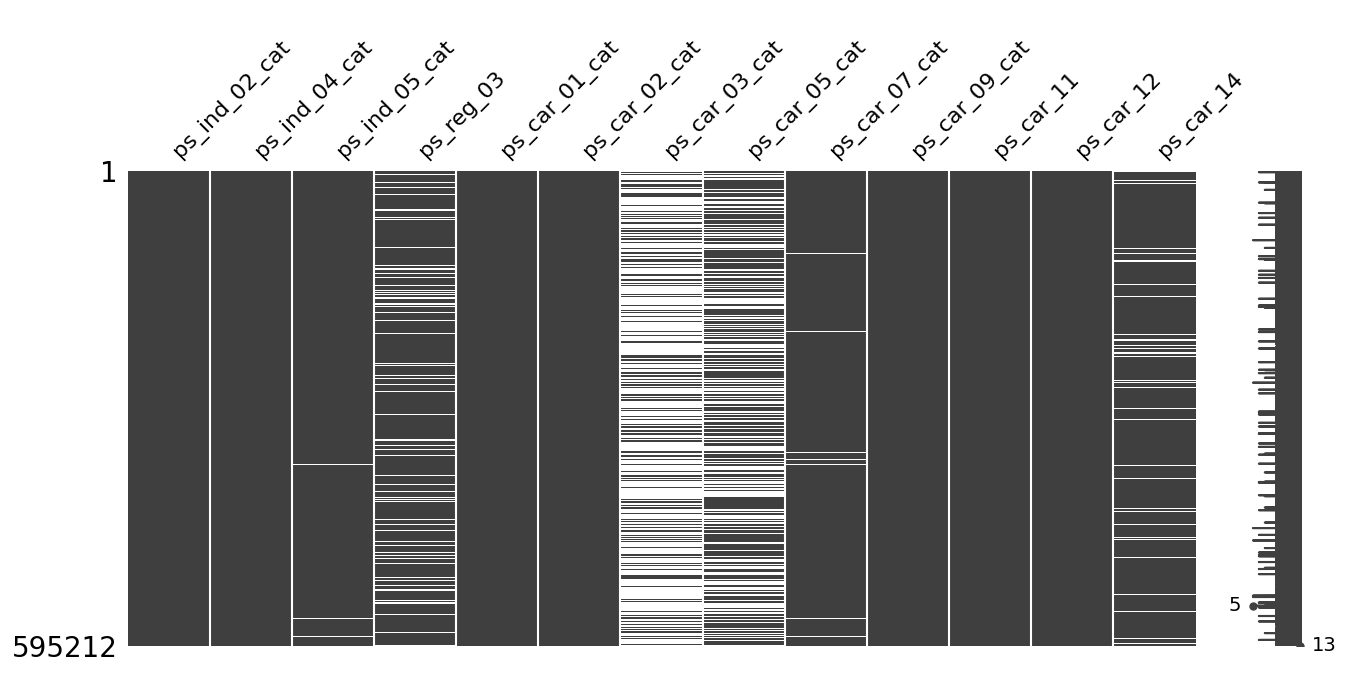
\includegraphics[width=\textwidth]{attrib_analysis}
\end{figure}

\subsection{Analiza danych}
Po wstępnej analizie danych odkryliśmy, że w zbiorze danych posiadamy około 79\% niekompletnych wierszy. Rysunek \ref{attrib_analysis} przedstawia pokrycie niekompletnych atrybutów - jest ich jedynie 13, z czego większość jest wybrakowana w bardzo niewielkim stopniu.

Największym winowajcą jest atrybut binarny \textsl{ps\_car\_03\_cat}, którego brakuje aż w 70\% wierszy, oraz atrybut \textsl{ps\_car\_05\_cat} (brakuje go w 44\% przypadków).

\subsection{Uzupełnienie brakujących danych}
W związku z powyższym, planujemy uzupełnić brakujące atrybuty na bazie kompletnych wierszy danych. Do tego zastosujemy bibliotekę pythonową \textsl{impyute}, ale nie będziemy analizować, jaka jest zależność między konkretnymi metodami interpolacji wybrakowanych atrybutów a hiperparametrami trenowanego klasyfikatora - ręcznie wybierzemy tą, która daje najlepsze (i najszybsze) rezultaty.

\subsection{Alternatywne dane}
Końcową wersję naszego algorytmu heurystycznego planujemy przetestować przy użyciu dodatkowego zbioru danych dot. przewidywania bankructwa polskich firm, który analizowaliśmy w \href{https://github.com/przestaw/Data_Mining_Bancrupcy}{innym projekcie}.


\section{Propozycja rozwiązania}
////////////////TODO: chyba faktycznie weźmy algo wspinaczkowy z tabu i bez plus może jeszcze jakiś jeden na pałę, dla porównania - IMO genetyczny jakiś

\section{Funkcja celu}
///////////////TODO: skoro mamy firme ubezpieczeniową, to Expected cost jest chyba najlepszy, tu jest ladnie opisany:
https://www.svds.com/the-basics-of-classifier-evaluation-part-1/

Expected cost = p(p) × [ p(true positive) × benefit(true positive)
                        + p(false negative) × cost(false negative) ]
              + p(n) × [ p(true negative) × benefit(true negative)
                        + p(false positive) × cost(false positive) ]
                        
Pewnie przydaloby sie znalezc jakies typowy zysk na 1 rok z ubezpieczenia (zysk dla firmy) i sredni koszt wyplaty ubezpieczenia jednemu klientowi. 

\section{Sposób mierzenia jakości rozwiązania}
//////////////TODO: czy to nie dokladnie to samo co po prostu funkcja celu? czy moze chodzi o to zeby opisać jak sprawdzamy to (k-krotne walidacje itp.).
Chociaz deja napisal to \textsl{"sposobu mierzenia jakości rozwiązania (podsumowania wyników)."} i nie wiem co ma podsumowanie wynikow do tego sposobu mierzenia jakosci rozwiazania, moze ty lepiej zrozumiesz.
\end{document}